% Section 7.3 -- E3: classical baselines and the quantum comparison (P3)
% Numbers from results/baselines_timing.csv and results/E1_depth.csv (QAOA at p = 6).

\subsection{E3: Classical baselines and the quantum comparison}
\label{sec:e3}

E3 runs four classical methods on every instance: Karmarkar-Karp (KK) and greedy LPT, which balance load only and ignore conflicts by design, and simulated annealing (SA) and CP-SAT, which optimise the full cost in Section~\ref{sec:formulation}, conflicts included.
Sizes $n = 8, \dots, 20$ use the same ten instances as E1, so the classical and quantum results are directly comparable; $n = 21, \dots, 28$ use one instance each, since repeating the exact reference ten times over is the slow part, not the baselines themselves.
The reference optimum is brute force up to $n = 24$ and CP-SAT above it (Section~\ref{sec:setup}).

\begin{figure}[p]
  \centering
  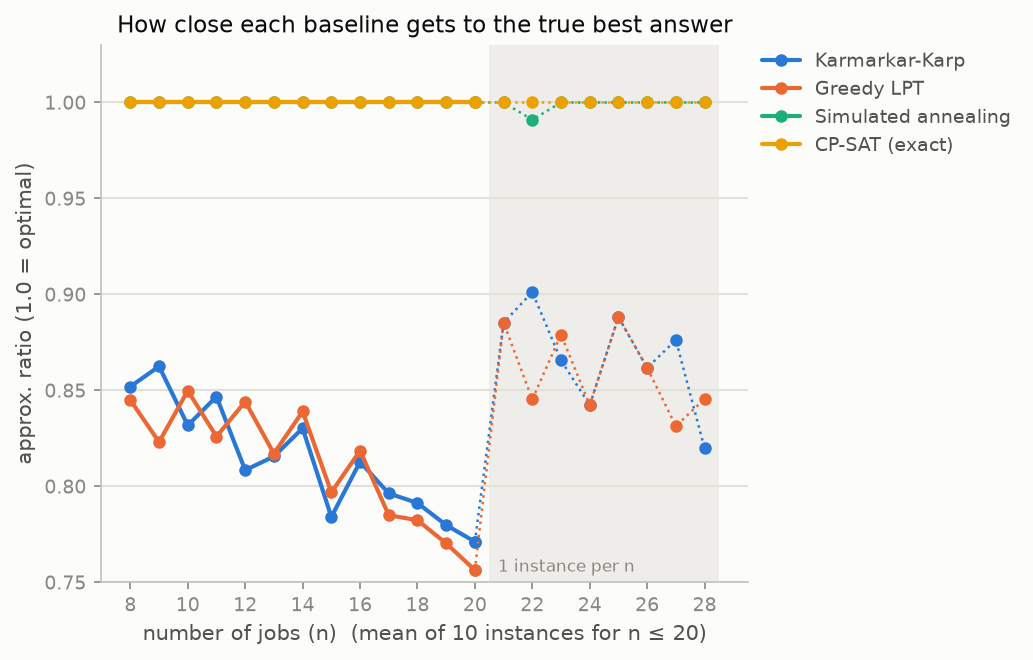
\includegraphics[width=0.8\linewidth]{baseline_approx_ratio.png}\\[6pt]
  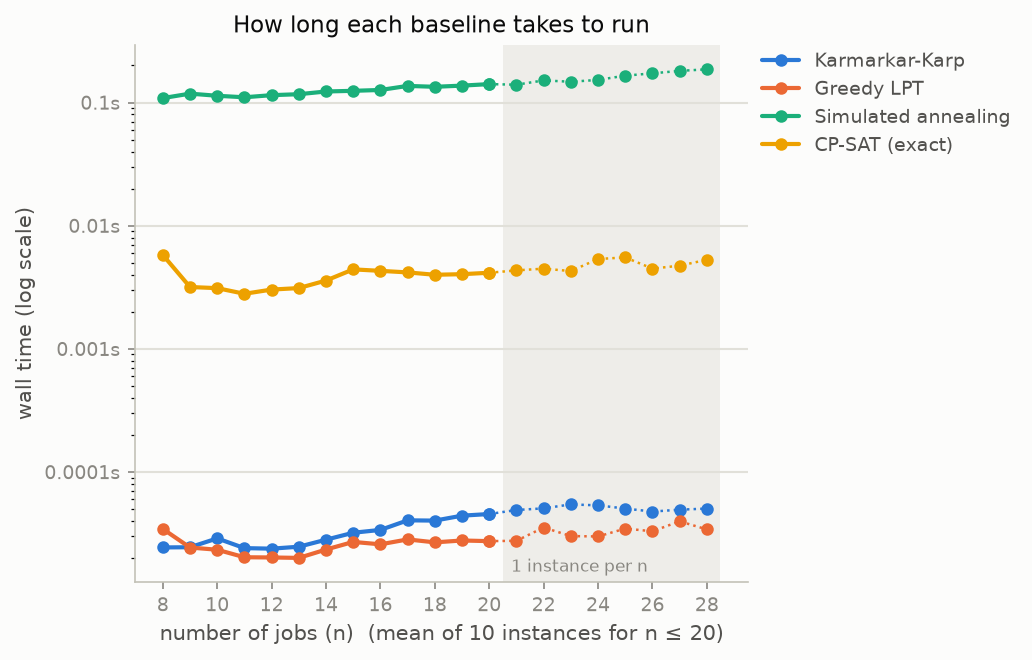
\includegraphics[width=0.8\linewidth]{baseline_wall_time.png}
  \caption{E3. Top: approximation ratio of each baseline's solution. Bottom: wall time (log scale). The shaded region past $n = 20$ has one instance per size rather than ten.}
  \label{fig:e3-baselines}
\end{figure}

KK and LPT land at $0.82$ and $0.81$ on average, with no clear trend in $n$ (Fig.~\ref{fig:e3-baselines}, top): since both ignore the conflict graph, their quality is set entirely by how evenly the balance term happens to split the planted weights, which does not get easier or harder as $n$ grows.
SA and CP-SAT are both effectively exact: CP-SAT finds the true optimum at every size by construction, and SA reaches a ratio of $1.0000$ at 136 of 138 runs, falling to $0.991$ at its worst.
This gap matters for conflicts specifically (Fig.~\ref{fig:e3-violations}): KK and LPT leave a mean of $5.06$ and $5.12$ violated edges per solution, while SA and CP-SAT leave $0.065$ and $0.058$, and find a fully conflict-free schedule on $93.5\,\%$ and $94.2\,\%$ of instances respectively -- consistent with $\lambda = 0.5$ being calibrated for roughly $90\,\%$ zero-violation optima (Section~\ref{sec:formulation}).

\begin{figure}[t]
  \centering
  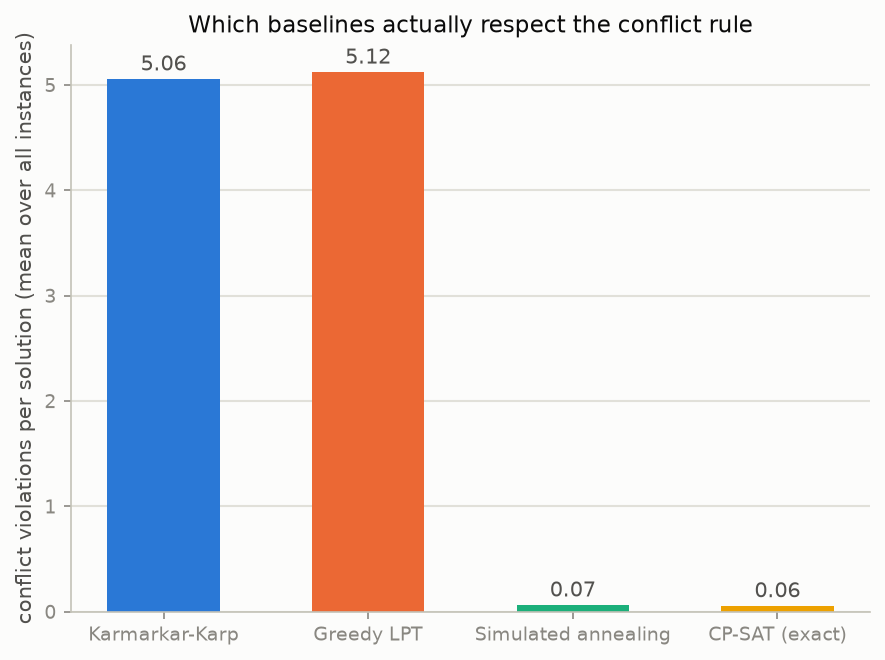
\includegraphics[width=0.6\linewidth]{baseline_violations.png}
  \caption{E3. Mean conflict violations per solution, averaged over all instances and sizes. KK and LPT never look at the conflict graph; SA and CP-SAT do.}
  \label{fig:e3-violations}
\end{figure}

Speed separates the two exact-ish methods sharply (Fig.~\ref{fig:e3-baselines}, bottom).
KK and LPT finish in tens of microseconds.
CP-SAT, despite being exact, is almost as fast: a mean of $3.9$\,ms and a worst case of $31$\,ms, including $5.3$\,ms to prove the optimum at $n = 28$.
SA is the slowest baseline at a mean of $126$\,ms, because it always runs its full $20{,}000$-iteration cooling schedule regardless of $n$, while CP-SAT's branch-and-cut exploits the structure of these instances directly.

\begin{figure}[t]
  \centering
  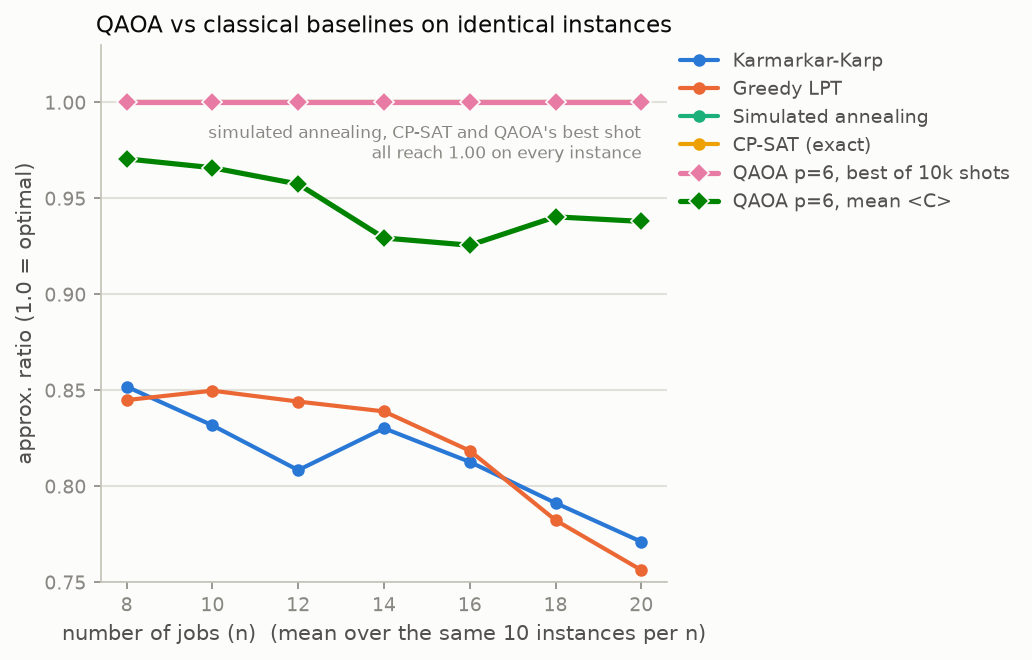
\includegraphics[width=0.8\linewidth]{qaoa_vs_baselines.png}
  \caption{QAOA's best depth ($p = 6$) against all four baselines, at the sizes where both have data ($n = 8$--$20$).}
  \label{fig:qaoa-vs-baselines}
\end{figure}

This answers RQ2 directly (Fig.~\ref{fig:qaoa-vs-baselines}).
QAOA at $p = 6$ beats both KK and LPT at every size tested, with approximation ratios of $0.93$--$0.97$ against $0.76$--$0.85$.
It never beats SA or CP-SAT, which reach $1.0000$ at every size by construction.
So QAOA is clearly doing more than naive load balancing, but at these sizes the gap to the strongest classical methods is not closed, and CP-SAT solves the whole problem, exactly, in milliseconds -- the scope set out in Section~\ref{sec:intro}: no quantum advantage here, by design, not by accident.
